\documentclass[12pt, a4paper, oneside]{article}
\usepackage{graphicx}
\usepackage{arial}
\renewcommand{\familydefault}{\sfdefault}
\usepackage[T1]{fontenc}
\usepackage[polish]{babel}
\usepackage[utf8]{inputenc}
\usepackage{lmodern}
\usepackage[left=2cm,right=2cm,top=2cm,bottom=2cm]{geometry}
\selectlanguage{polish}
\usepackage{booktabs, multicol, multirow}
\usepackage{longtable}
\usepackage{textcomp}
\usepackage{slashbox}
\begin{document}
\begin{titlepage}
\vspace*{7\baselineskip}
\begin{center}
{\Huge MEDIA TRANSMISYJNE 2}
\end{center}
\vspace*{\baselineskip}
\begin{center}
{\Large PROJEKT 2}
\end{center}
\vspace*{5\baselineskip}
{\it TYTUŁ PROJEKTU:}
\begin{center}
{\bf\large Wyznaczanie zasięgu stacji bazowej sieci trankingowej (450 MHz) zlokalizowanej w~punkcie o współrzędnych: 20\textdegree 24’47”E, 49\textdegree 43’05”N (Limanowa).} 
\end{center}
\vspace*{10\baselineskip}
\raggedleft
TERMIN: WTOREK 11:15\\
AUTOR: IGOR MICHALSKI
\end{titlepage}
\section{Wstęp}
\indent\indent Przy wykorzystaniu programu „Mapki” (MTV) oraz „Piast” (dla porównania) wyznaczony zostanie zasięg stacji bazowej sieci trankingowej (450 MHz) zlokalizowanej w punkcie o współrzędnych: 20\textdegree 24’47”E, 49\textdegree 43’05”N (Limanowa). Antena stacji bazowej zawieszona jest na wysokości 40 m od stopy masztu. Wysokość stopy masztu wynosi 392 m n.p.m. Zysk energetyczny anteny G$_{max}$~=~8~dBi. Antena ma dookólną charakterystykę. Zastępcza moc promieniowana izotropowo równa się~16~dBW. Stacja pracuje na trzech kanałach: 5, 32 i 42. (f$_{kan}$ = 428,5 + (kan - 1) $\cdot$ 0,0125 MHz). Określony zostanie azymut maksymalnego i minimalnego  zasięgu  stacji,  jeśli  wartość  graniczna natężenia  pola  zapewniająca  poprawną łączność wynosi 22 dB$\mu$V/m na wysokości 1,5 m (stosując poprawkę height gain zawartą w ITU P.370-7). Dla punktów wyznaczających zasięg wyznaczony zostanie także profil terenu.
\section{Obliczenia własne}
\subsection{Poprawka height gain}
\indent\indent Realizacja projektu z wykorzystaniem programu ,,Mapki'' wymagała wyznaczenia poprawki height gain, która w rekomendacji ITU-R P-370.7 opisana jest wzorem:
\begin{equation}
HG = \frac{c}{6}\cdot20~ log_{10}(\frac{h_2}{10}),
\end{equation}
gdzie:
\begin{itemize}
\item $c$ - współczynnik zależny od częstotliwości oraz zabudowy terenu,
\item $\frac{h_2}{10}$ - wysokość zawieszenia anteny odbiorczej nad powierzchnią terenu, względem wysokości wyjściowej 10 metrów.
\end{itemize}
\indent\indent Z rekomendacji ITU-R P.370-7 wybrany został współczynnik $c$ = 6 dB. Odpowiada on zakresowi fal UHF (300 - 3000 MHz) w strefie podmiejskiej. Taki wybór jest optymalny dla warunków propagacyjnych w miejscowości o zabudowie niskiej i średnio gęstej, jaka występuje w Limanowej. Zakładana w projekcie wysokość $h_1 = 1,5$ m n.p.t., a poprawka wyznaczona zostanie względem $h_2 = 10$ m n.p.t. Po podstawieniu otrzymano:
\begin{equation}
HG=\frac{6}{6}\cdot 20~log_{10}(\frac{1.5}{10})=-16,48~[dB]
\end{equation}
\indent\indent Antena odbiorcza w symulacji umieszczona została na wysokości 10 m, gdzie poziom odebranego sygnału jest znacznie wyższy. Aby to skompensować należy wyznaczoną wartość $HG$ odjąć od minimalnej wartości pola elektrycznego, która zapewnia poprawną łączność, tj. 22 db$\mu$V/m - zgodnie z założeniami projektu. Otrzymano:
\begin{equation}
E_{min} = 22~db\mu V/m + 16,48~dB = 38,48~dB\mu V/m=39~dB\mu V/m
\end{equation}
Wartość $E_{min}$ została zaokrąglona w górę, ponieważ w programie ,,Mapki'' nie można wprowadzić liczb zmiennoprzecinkowych, a zaokrąglenie w dół spowodowałoby przekłamanie, skutkujące rzeczywistym brakiem zasięgu na wysokości 1.5 m, pomimo wyników symulacji wskazujących na dostateczny poziom sygnału do nawiązania połączenia.
\subsection{Moc nadajnika}
\begin{equation}
EIRP=16~dBW \Rightarrow P = 40~W=0,04~kW
\end{equation}
\section{Symulacje wykonane programem ,,Mapki''}
\indent\indent Z powodu niedokładności mapy zaimplementowanej w programie, do obliczeń przyjęty został punkt najbliższy od zakładanego w projekcie. Ma on współrzędne geograficzne 20\textdegree 25’41”E, 49\textdegree 43’8”N i~znajduje się na terenie Limanowej. Tym samym zmieniła się też wysokość bezwzględna stopy masztu. Dla nowego położenia wynosi ona 459 m n.p.m.
\begin{figure}[h!]
\centering
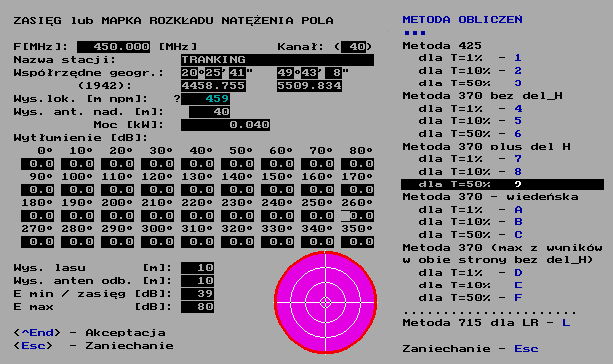
\includegraphics[scale=0.85]{pics/mapki/f1.png}
\caption{Częstotliwość, współrzędne geograficzne oraz wysokość zawieszenia anteny nadawczej, moc, wysokość zawieszenia anteny odbiorczej oraz E$_{min}$ (z uwzględnieniem poprawki HG) i E$_{max}$}
\end{figure}
\subsection{Zasięg minimalny}
\begin{figure}[h!]
\centering
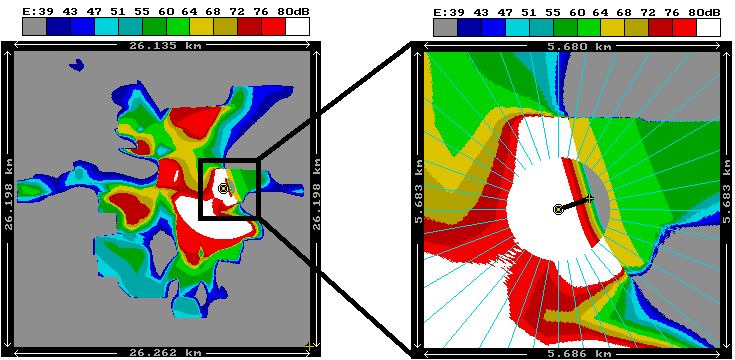
\includegraphics[scale=0.9]{pics/mapki/f2.png}
\caption{Mapa poziomu sygnału oraz powiększony fragment z naniesioną siatką azymutalną oraz ścieżką pomiędzy nadajnikiem (X) i odbiornikiem (+) dla E$_{min}$}
\end{figure}
\clearpage
\begin{figure}[h!]
\centering
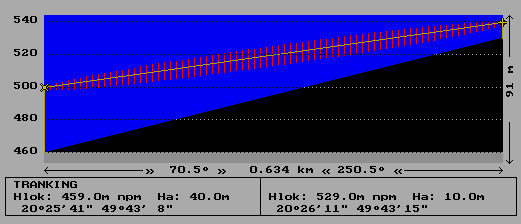
\includegraphics[scale=1.1]{pics/mapki/f3.png}
\caption{Profil terenu dla ścieżki zaznaczonej na rys. 2 (dla E$_{min}$)}
\end{figure}
Dzięki profilowi terenu można określić dokładny minimalny zasięg stacji nadawczej, a także sprawdzić przesłonięcie 1. strefy Fresnela, która w powyższym  przypadku jest całkowicie odsłonięta. Z rys. 2 oraz 3 wynika, że zasięg minimalny wynosi 634 m na azymucie 70\textdegree. Decydujący wpływ ma tutaj szybkie narastania zbocza góry.
\subsection{Zasięg maksymalny}
\begin{figure}[h!]
\centering
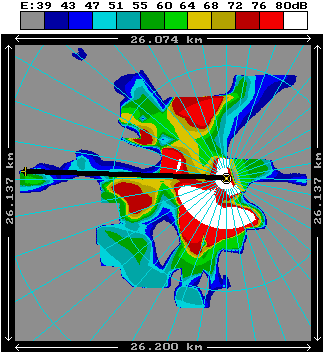
\includegraphics[scale=1.1]{pics/mapki/f4.png}
\caption{Mapa poziomu sygnału z naniesioną siatką azymutalną oraz ścieżką pomiędzy nadajnikiem (X) i odbiornikiem (+) dla E$_{max}$}
\end{figure}
\clearpage
\begin{figure}[h!]
\centering
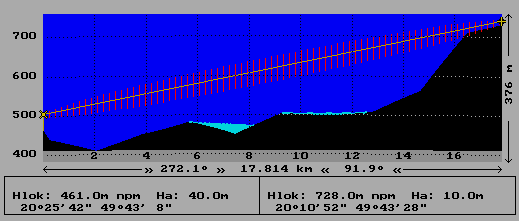
\includegraphics[scale=1.1]{pics/mapki/f5.png}
\caption{Profil terenu dla ścieżki zaznaczonej na rys. 4 (dla E$_{max}$)}
\end{figure}
Na tej trasie 1. strefa Fresnela jest prawie w całości odsłonięta. Dopiero w odległości około 16 km można zaobserwować niewielkie przesłonięcie od dołu przez wypukłość terenu. Zasięg maksymalny wynosi 17,814 km na azymucie 272\textdegree.
\section{Symulacje wykonane na platformie ,,Piast''}
\begin{figure}[h!]
\centering
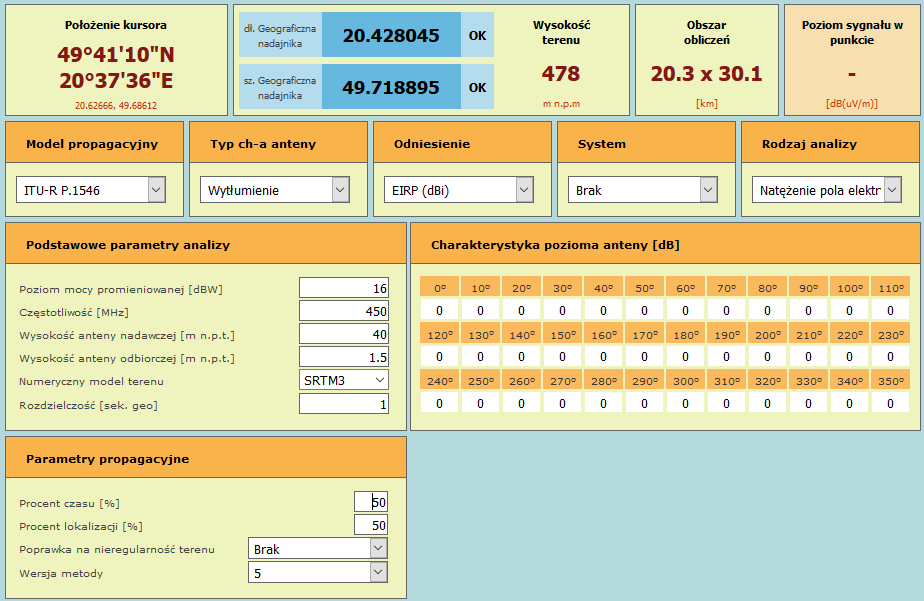
\includegraphics[scale=0.5]{pics/piast/f1.png}
\caption{Częstotliwość, współrzędne geograficzne oraz wysokość zawieszenia anteny nadawczej, moc promieniowana, wysokość zawieszenia anteny odbiorczej}
\end{figure}
\clearpage
\subsection{Zasięg minimalny}
\begin{figure}[h!]
\centering
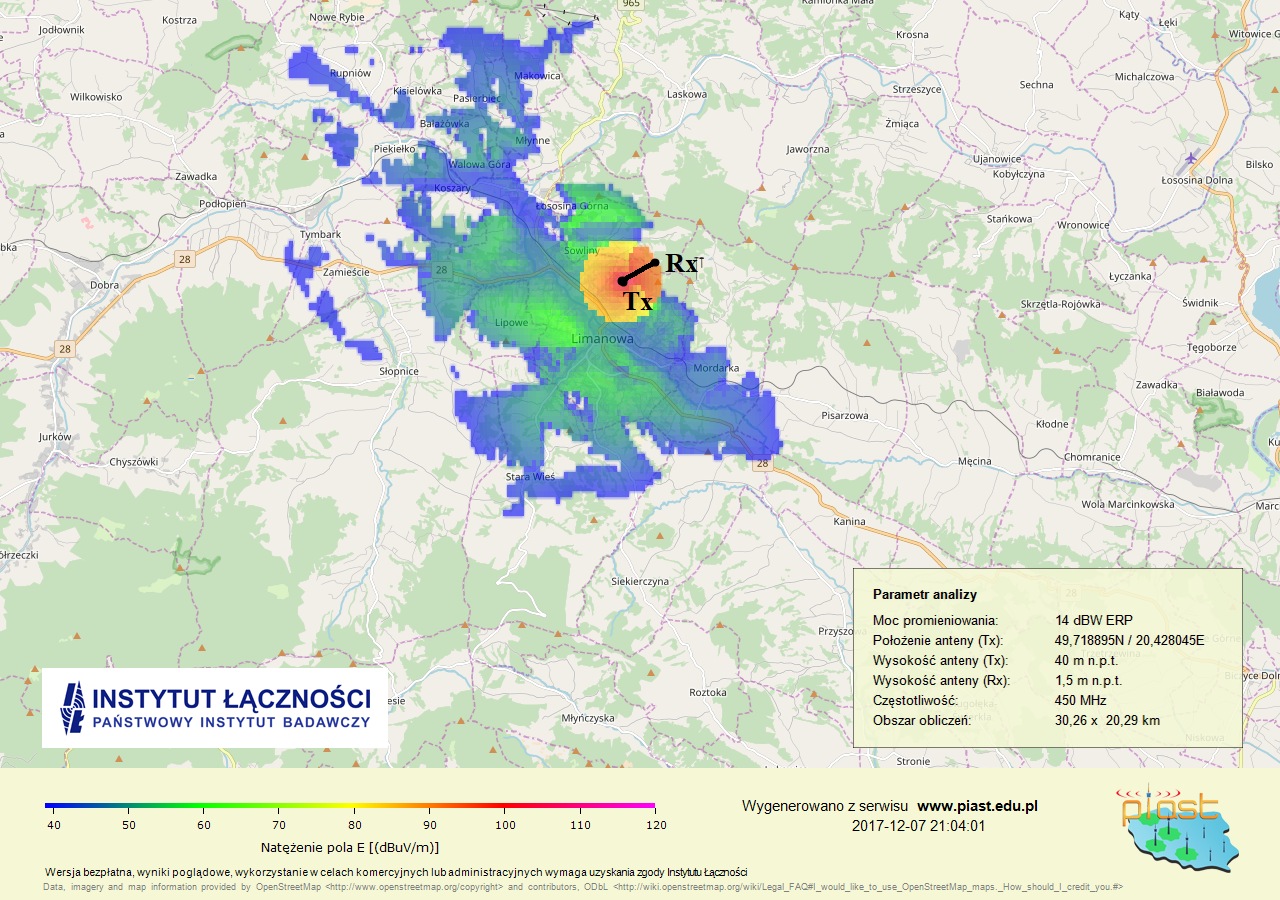
\includegraphics[scale=0.45]{pics/piast/f2.png}
\caption{Mapa poziomu sygnału oraz powiększony fragment z naniesioną ścieżką pomiędzy nadajnikiem (Tx) i odbiornikiem (Rx) dla E$_{min}$}
\end{figure}
\begin{figure}[h!]
\centering
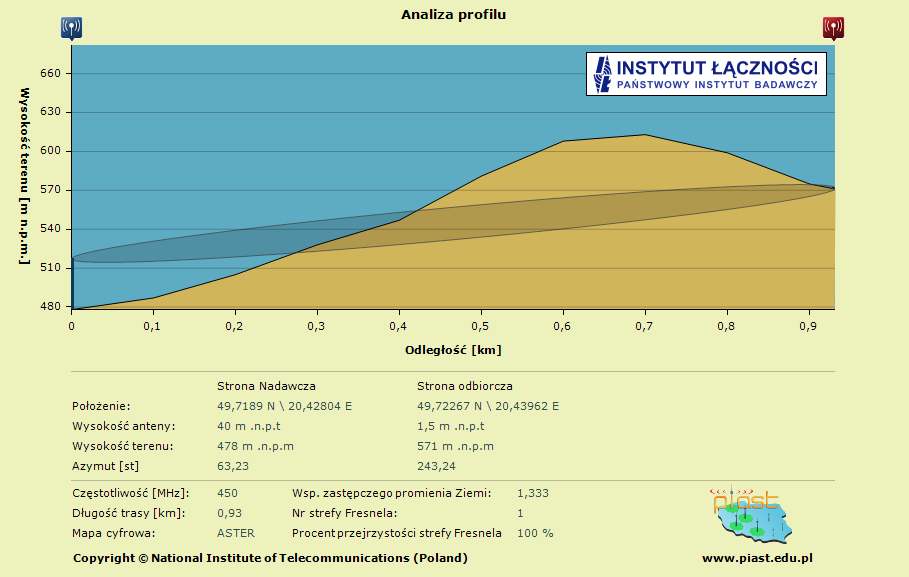
\includegraphics[scale=0.45]{pics/piast/f4.png}
\caption{Profil terenu dla ścieżki zaznaczonej na rys. 7 (dla E$_{min}$)}
\end{figure}
Wynik bardzo zbliżony do uzyskanego metodą ITU-R P.370-7. Szybko narastające zbocze góry mocno tłumi sygnał. Zasięg minimalny na azymucie 63,23\textdegree wynosi 930 m.
\clearpage
\subsection{Zasięg maksymalny}
\begin{figure}[h!]
\centering
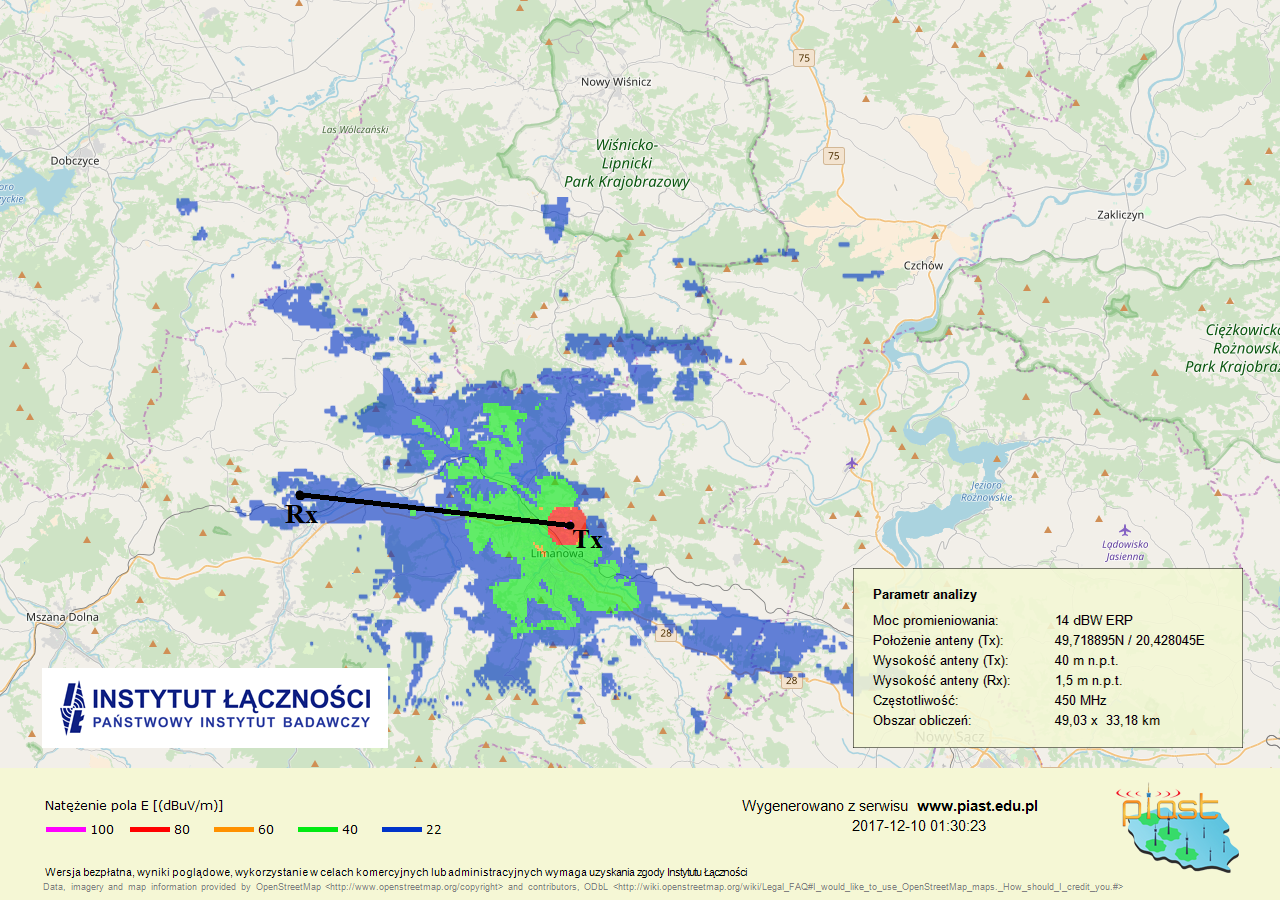
\includegraphics[scale=0.45]{pics/piast/f5.png}
\caption{Mapa poziomu sygnału oraz powiększony fragment z naniesioną ścieżką pomiędzy nadajnikiem (Tx) i odbiornikiem (Rx) dla E$_{max}$}
\end{figure}
\begin{figure}[h!]
\centering
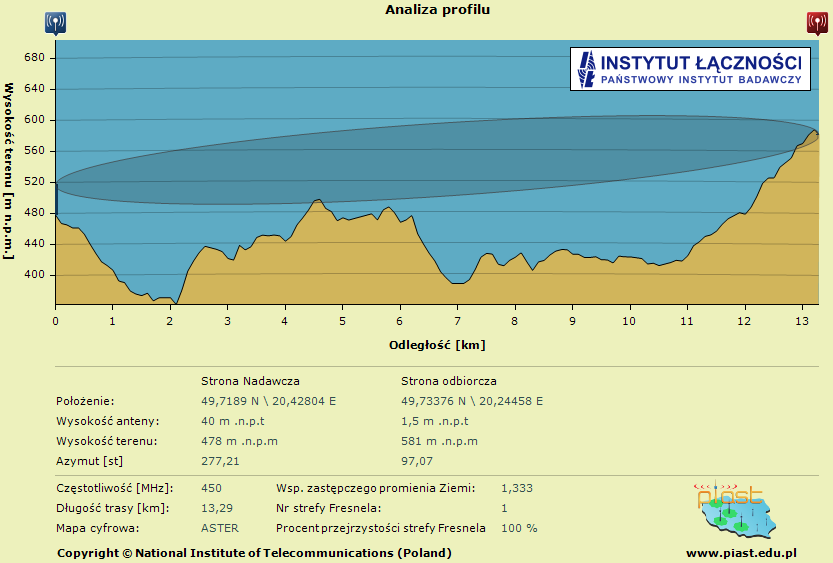
\includegraphics[scale=0.6]{pics/piast/f3.png}
\caption{Profil terenu dla ścieżki zaznaczonej na rys. 9 (dla E$_{max}$)}
\end{figure}
Rezultat znacznie różniący się od uzyskanego w programie ,,Mapki''. Znacząco zmniejszył się zasięg na azymucie około 180\textdegree - 280\textdegree. Zasięg maksymalny wynosi 5,27 km na azymucie 209,37\textdegree.
\clearpage
\section{Podsumowanie}
% Table generated by Excel2LaTeX from sheet 'Arkusz1'
\begin{table}[h!]
  \centering
  \caption{Porównanie zasięgów: maksymalnego i minimalnego dla ,,Mapek'' i ,,Piasta''}
    \begin{tabular}{|c|c|c|c|c|}\hline
    \backslashbox{ Parametr }{ Program } & \multicolumn{2}{c}{\textbf{Mapki}} & \multicolumn{2}{|c|}{\textbf{Piast}} \\\hline
    \multicolumn{5}{|c|}{\textbf{Zasięg minimalny}} \\\hline
    {Azymut [\textdegree]} & \multicolumn{2}{c}{70} & \multicolumn{2}{|c|}{63,23} \\\hline
    {Dystans [km]} & \multicolumn{2}{c}{0,634} & \multicolumn{2}{|c|}{0,93} \\\hline
    \multicolumn{5}{|c|}{\textbf{Zasięg maksymalny}} \\\hline
    {Azymut [\textdegree]} & \multicolumn{2}{c}{272} & \multicolumn{2}{|c|}{209,37} \\\hline
    {Dystans [km]} & \multicolumn{2}{c}{17,814} & \multicolumn{2}{|c|}{5,27} \\\hline
    \end{tabular}%
  \label{tab:addlabel}%
\end{table}%
\indent Wyniki symulacji z wykorzystaniem metody ITU-R P.370 przedstawiają znacznie bardziej optymistyczne rezultaty, niż dla ITU-R P.1546. Zasięg maksymalny dla pierwszej z wymienionych metod jest większy o ponad 12 km, czyli o ponad 3 razy. Znaczące różnice w pokryciu terenu widoczne są na wszystkich azymutach, przy dystansie większym niż około 4 - 5 km. Dla mniejszych odległości, obiema metodami otrzymano podobne pokrycie, jednak poziomy sygnału wyznaczone metodą P.1546 są niższe średnio o około 10 - 20 dB. Zasięgiem pokryte zostało całe miasto Limanowa, a także prawie w całości gmina Limanowa. Lokalizacja nadajnika znacznie utrudniała propagacje sygnału na azymucie 50\textdegree - 100\textdegree. Znajduje się tam strome zbocze góry, które skutecznie ogranicza propagację fal - całkowicie dla metody używanej na platformie ,,Piast'' i częściowo dla metody w programie ,,Mapki''. Obecnie metoda ITU-R P.370 jest już wycofana z użytku, natomiast ITU-R P.1546 jest powszechnie używana przy planowaniu systemów radiowych. Tym samym należy uznać ją za bardziej wiarygodną, a wyniki otrzymane z programu ,,Mapki'' traktować jedynie jako przybliżenie.
\begin{figure}[h!]
\centering
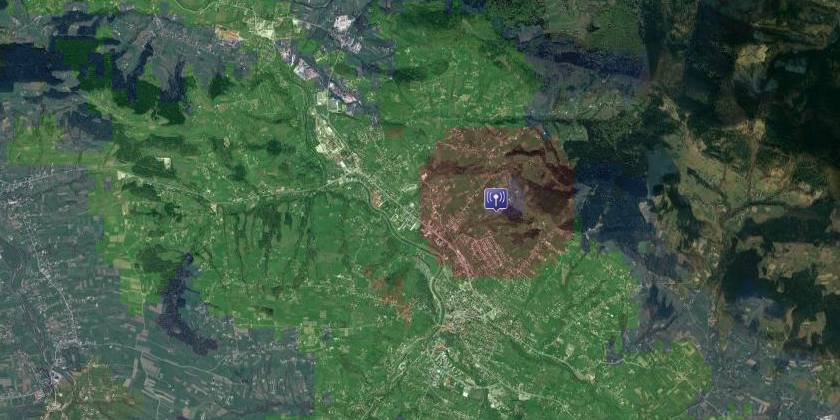
\includegraphics[scale=0.6]{pics/piast/f6.png}
\caption{Pokrycie miasta Limanowa, w miejscach niepokolorowanych sygnał poniżej E$_{min}$, zdjęcie satelitarne z platformy ,,Piast''}
\end{figure}
\end{document}